\chapter{Design and Implementation PhylogenyUz}

\section*{}

In this chapter, discussed about PhylogenyUz, which 
is phylogenetic analysis system and considered to 
be a solution to the challenge. Also, discussed 
about used technologies, system advantages and 
disadvantages. Given User-Manual for user and scientists
and instructions for developers.

\section{Developing software to analyze taxons}

To solve given problem we have to develop software, 
which uses algorithms of estimate calculations to 
reconstruct phylogenetic tree.

It has to be user-friendly, efficient, 
responsive and cross platform. Also, it is multilingual, 
can be used English and Uzbek languages in UI.

To achieve this we use Java programming language. 
Because, Java needs only Java Virtual Machine to run.
More about system requirements given in the next sections.

Main idea is to integrate algorithms of estimate calculations
and existing methods of reconstruction.
For that, used biojava3 \cite{biojava} library, which is 
open-source library, written by developers in 
bioinformatics and has many implementations of 
existing methods.

We name our software PhylogenyUz.
Below given diagram \ref{img:workflow1} of major actions what 
user can do in PhylogenyUz.

PhyloWidget \cite{phylowidget} 
used as a framework for the software which is
developed by Jordan and Piel.

\section{Design and overview of system components}

\subsection{Overview}
The purpose of this chapter is to present a detailed 
description of the PhylowidgetUz. It will explain the 
purpose and features of the system, the interfaces of 
the system, what the system will do, the constraints 
under which it must operate and how the system 
will react to external stimuli. This document is intended 
for both the users and the developers of the system 
and will be proposed to the biology scientists for its approval.

You can see below \ref{img:workflow1} the overall architecture of the program.

\begin{figure}[!htbp] 
  \center
  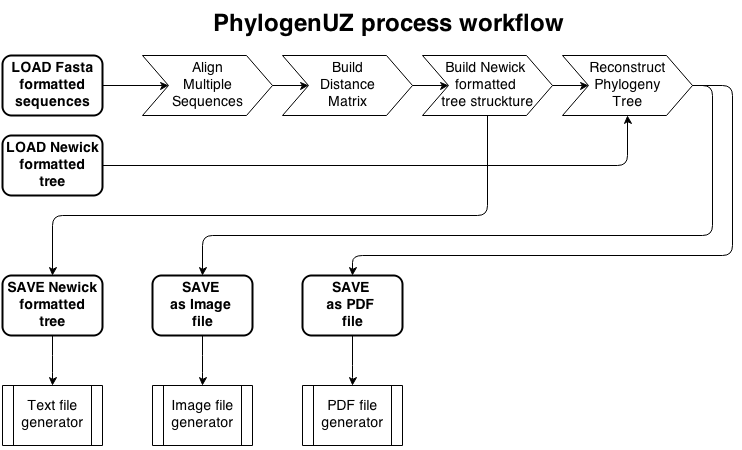
\includegraphics[width=1\textwidth]{workflow.png}
  \caption[w]{Process workflow for reconstructing 
  phylogenetic tree in PhylogenUz} 
  \label{img:workflow1}  
\end{figure}

\subsubsection{Installation and Run PhylogenyUz}
No need to install the software. To start you 
need to just run in the console command:

\textit{java -jar PhylogenUz.jar}.

This can cause discomfort for the user who is used to run 
the program by clicking in the windows operating system.

To solve this problem in the next releases, we want 
to create separate versions for linux and for 
windows operation systems.

\subsection{General features of PhylogenyUz}

\subsubsection{Creating New tree \ref{img:p1}}
By default, PhylogenyUz creates a new phylogenetic tree on startup.
If you want to create a new tree, you need to select New Tree item menu from 
context menu File or use Ctrl+N shortcuts.
Then, PhylogenyUz shows basic node on main view.

\begin{figure}[!htbp] 
  \center
  \includegraphics[width=0.8\textwidth]{p1.png}
  \caption[w]{Creating new phylogenetic tree in PhylogenUz} 
  \label{img:p1}  
\end{figure}

\subsubsection{Loading Fasta formated files}
By default, PhylogenyUz reads Fasta \cite{fasta} formatted 
phylogeny sequences. To do that, one needs to select Load Fasta 
file item menu from context menu File or use Ctrl+F shortcuts.

As soon as, reading completed, PhylogenyUz alignes all sequences,
calculates distance matrix, generates Newick formatted tree and 
shows on main view.

\begin{figure}[!htbp] 
  \center
  \includegraphics[width=1\textwidth]{p2.png}
  \caption[w]{Loading fasta formatted files in PhylogenUz} 
  \label{img:p2}  
\end{figure}

\subsubsection{Loading Phylogenetic Trees}
PhylogenyUz reads Newick \cite{newick}, Nexus or NHX formatted tree files.
To load tree files, select Load Tree menu item from context menu File.
PhylogenyUz reconstructs phylogenetic tree immediately without 
any calculation and shows on main view.

\begin{figure}[!htbp] 
  \center
  \includegraphics[width=1\textwidth]{p3.png}
  \caption[w]{Loading phylogenetic tree in PhylogenUz} 
  \label{img:p3}  
\end{figure}

\begin{figure}[!htbp] 
  \center
  \includegraphics[width=0.5\textwidth]{p31.png}
  \caption[w]{Open file Dialog} 
  \label{img:p31}  
\end{figure}

\subsubsection{Saving Phylogenetic Trees}
PhylogenyUz saves Newick \cite{newick} formatted tree files.
To save tree files, select Save Tree menu item from context menu File.
It saves tree from main view.  

\begin{figure}[!htbp] 
  \center
  \includegraphics[width=1\textwidth]{p4.png}
  \caption[w]{Saving phylogenetic tree in PhylogenUz} 
  \label{img:p4}  
\end{figure}

\begin{figure}[!htbp] 
  \center
  \includegraphics[width=0.5\textwidth]{p41.png}
  \caption[w]{Save Dialog} 
  \label{img:p41}  
\end{figure}

\subsubsection{Saving as Image or PDF}
By using this sub menus you can save 
phylogenetic tree as a image file or PDF file.
 
\begin{figure}[!htbp] 
  \center
  \includegraphics[width=0.8\textwidth]{p5.png}
  \caption[w]{Saving as Image or PDF} 
  \label{img:p5}  
\end{figure}

\subsubsection{Render type}
By default, Phylogeny displays phylogenetic trees in 
rectangular form. But user can change render type 
by selecting menu item Renderer Type from context menu View.
It supports 3 types of rendering: Rectangular, Diagonal and Circular.
Shurtcuts are Ctrl+1, Ctrl+2 and Ctrl+3 respectively.

\begin{figure}[!htbp] 
  \center
  \includegraphics[width=0.8\textwidth]{p6.png}
  \caption[w]{Rectangular render type} 
  \label{img:p6}  
\end{figure}

\begin{figure}[!htbp] 
  \center
  \includegraphics[width=0.8\textwidth]{p7.png}
  \caption[w]{Diagonal render type} 
  \label{img:p7}  
\end{figure}

\begin{figure}[!htbp] 
  \center
  \includegraphics[width=0.8\textwidth]{p8.png}
  \caption[w]{Circular render type} 
  \label{img:p8}  
\end{figure}

\subsubsection{Styling options}
User can change rendering styles as Text Multiplier,
Text Angel, Node Size, Line Weight, Render Threshold,
Text Size, Stretch Tree and Branch Lengths.

Also, PhylogenyUz can manage tree structure. 
User can use features as Flip Tree, Enforce Unique Labels, 
Auto-sort Tree and Remove Elbows.

\subsubsection{Search}
Search feature is very useful to find and highlight tree nodes by keyword.
Enter keyword into search input box and PhylogenyUz 
highlights all matched nodes.

\begin{figure}[t] 
  \center
  \includegraphics[width=0.8\textwidth]{p9.png}
  \caption[w]{Search} 
  \label{img:p9}  
\end{figure}

\section{System Requirements Specification}

\subsection{Introduction}
The section introduces the system requirements specification (SRS) 
for the PhylogenyUz (PU) system to its readers.

\subsection{Specification Definition}
This specification documents the system-level 
requirements for the PU system.

\subsection{Specification Objectives}
The objectives of this specification of the PU are to:

- Provide a system overview of the PU including definition, 
goals, objectives, context, and major capabilities.

- Functional requirements.

- Data requirements.

- Quality requirements.

- Constraints.

\subsection{Intended Audiences}

The intended audiences of stakeholders for this 
specification of the PU include:

- Biology scientists.

- Biology researches.

- Users, who are any private individuals that take part in a biology held in the PU.

\subsection{External Software}

The system requires Java 1.6 or newer version.

\subsection{Input formats}

\subsubsection{Fasta format \cite{fasta}}
A sequence in FASTA format begins with a single-line description, 
followed by lines of sequence data. The description line is 
distinguished from the sequence data by a greater-than ("$>$") 
symbol in the first column. The word following the "$>$" symbol 
is the identifier of the sequence, and the rest of the line is 
the description (both are optional). There should be no space 
between the "$>$" and the first letter of the identifier. 
It is recommended that all lines of text be shorter than 80 
characters. The sequence ends if another line starting 
with a "$>$" appears; this indicates the start of another 
sequence. A simple example of one sequence in FASTA format:
\begin{lstlisting}
>gi|5524211|gb|AAD44166.1| cytochrome b 
[Elephas maximus maximus]
LCLYTHIGRNIYYGSYLYSETWNTGIMLLLITMATAFMGYVLP
WGQMSFWGATVITNLFSAIPYIGTNLVEWIWGGFSVDKATLNR
FFAFHFILPFTMVALAGVHLTFLHETGSNNPLGLTSDSDKIPF
HPYYTIKDFLGLLILILLLLLLALLSPDMLGDPDNHMPADPLN
TPLHIKPEWYFLFAYAILRSVPNKLGGVLALFLSIVILGLMPF
LHTSKHRSMMLRPLSQALFWTLTMDLLTLTWIGSQPVEYPYTI
IGQMASILYFSIILAFLPIAGXIENY
\end{lstlisting}

\subsection{Output formats}

\subsubsection{Newick format \cite{newick}}
In mathematics, Newick tree format (or Newick notation or 
New Hampshire tree format) is a way of representing graph-theoretical 
trees with edge lengths using parentheses and commas. 

\begin{lstlisting}
(,,(,));                               no nodes are named
(A,B,(C,D));                           leaf nodes are named
(A,B,(C,D)E)F;                         all nodes are named
(:0.1,:0.2,(:0.3,:0.4):0.5);           all but root node have a distance to parent
(:0.1,:0.2,(:0.3,:0.4):0.5):0.0;       all have a distance to parent
(A:0.1,B:0.2,(C:0.3,D:0.4):0.5);       distances and leaf names (popular)
(A:0.1,B:0.2,(C:0.3,D:0.4)E:0.5)F;     distances and all names
((B:0.2,(C:0.3,D:0.4)E:0.5)F:0.1)A;    a tree rooted on a leaf node (rare)
\end{lstlisting}

- Tree: The full input Newick Format for a single tree\par
- Subtree: an internal node (and its descendants) or a leaf node\par
- Leaf: a node with no descendants\par
- Internal: a node and its one or more descendants\par
- BranchSet: a set of one or more Branches\par
- Branch: a tree edge and its descendant subtree.\par
- Name: the name of a node\par
- Length: the length of a tree edge.\par

\subsection{Nexus format}
Nexus file format (usually .nex or .nxs) is widely used 
in Bioinformatics. Several popular phylogenetic programs 
such as Paup*, MrBayes, Mesquite, and MacClade use this format.

Command inside square brackets $[$ and $]$ are ignored (comment). 
Each block starts with BEGIN block_name; and finishes with END;

Example 1:\par
\begin{lstlisting}
#NEXUS
Begin data;
Dimensions ntax=4 nchar=15;
Format datatype=dna symbols="ACTG" missing=? gap=-;
Matrix
Species1   atgctagctagctcg
Species2   atgcta??tag-tag
Species3   atgttagctag-tgg
Species4   atgttagctag-tag           
;
End;
\end{lstlisting}
Example 2:\par
\begin{lstlisting}
#NEXUS
#BEGIN TAXA;
  TAXLABELS A B C;
END;

BEGIN TREES;
  TREE tree1 = ((A,B),C);
END;
\end{lstlisting}

\addcontentsline{toc}{section}{\numberline{}Conclusion for Chapter 3}
\section*{Conclusion for Chapter 3}

- Integration algoritms of estimate colculations into
reconstructing phylogenetic tree increases quality of results.

- Developed software PhylogenyUz can be used to 
reconstruct phylogenetic trees.

- Open-source library BioJava has wide scope to analyze
phylogenetic data.

\newpage